
\section{Results and Analysis}
\subsection{1-Site Model}
The 1-Site model is the simplest version of the Hubbard-Model as it requires no hopping term and has only 4 states and can be compared to the exact results.
\subsubsection{Comparison $N$ and $N_t$}
\begin{figure}[H]
	\centering
	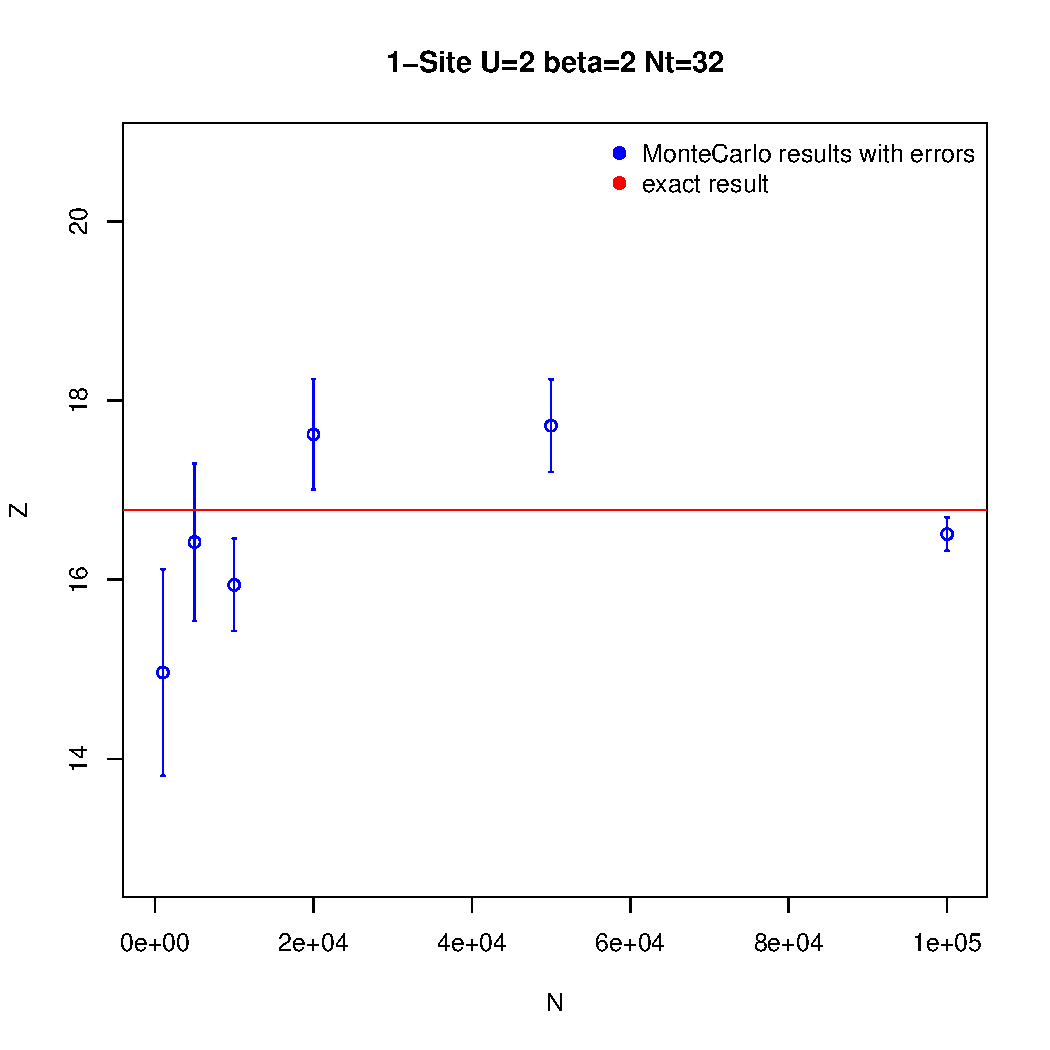
\includegraphics[width=0.5\linewidth]{figs/plot_Z1N}
	\caption[Scaling of Z with N]{This plot shows the result of Z with $U=2$, $\beta=2$ and $N_t=32$ for different numbers of samples.}
	\label{fig:plotz1n}
\end{figure}
Figure \ref{fig:plotz1n} shows how the result depends on the number of samples we average over. While the true accuracy gets slightly better it is clear that the calculated bootstrap error, which gives the statistical error of the Monte-Carlo calculation, becomes smaller for more samples, as expected. The reason why our results are not more accurate is the systematical error from the Hubbard-Stratanovich/ Pathintegral approximation. This one can be improved by increasing the number of timeslices $N_t$.
\begin{figure}[H]
	\centering
	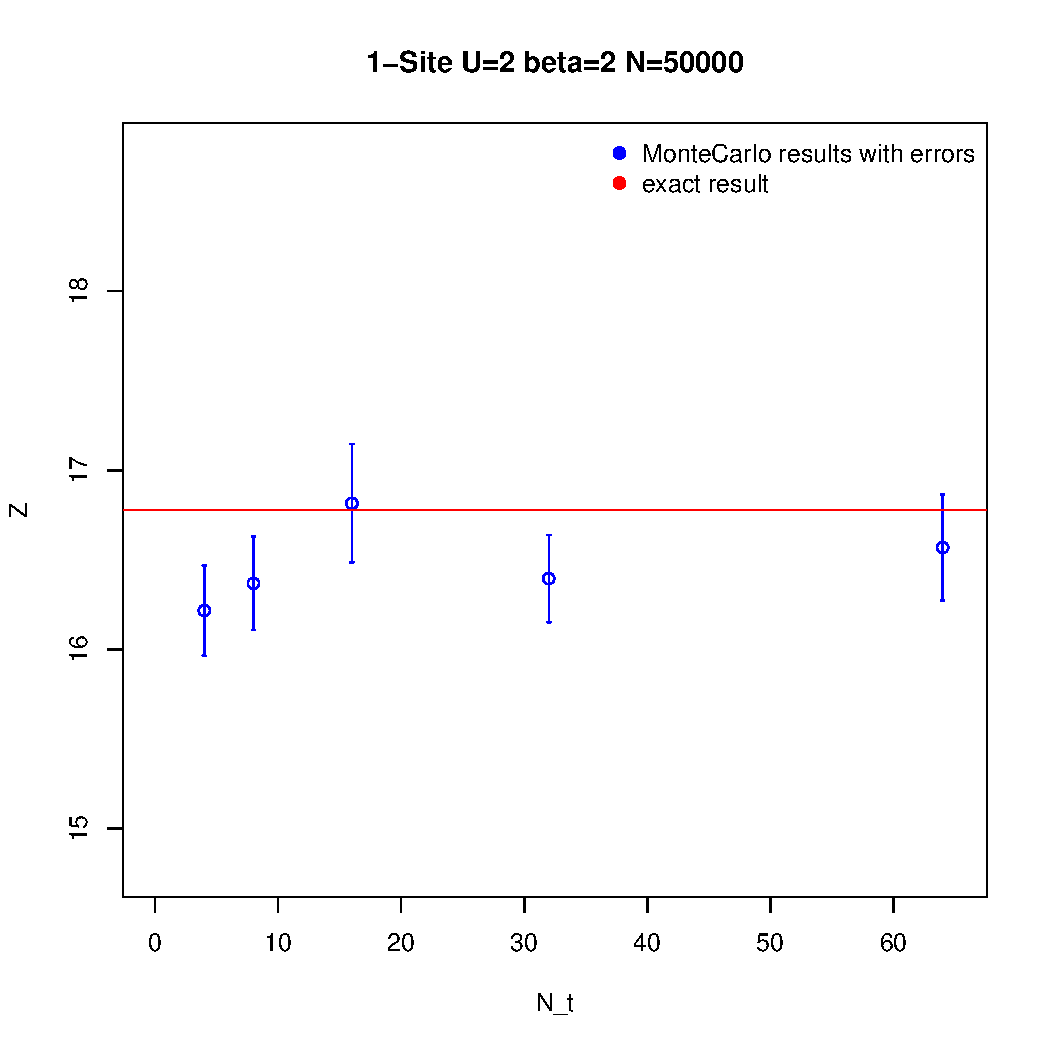
\includegraphics[width=0.5\linewidth]{figs/plot_Z1Nt}
	\caption[Scaling of Z with N_t]{This plot shows the result of Z with $U=2$, $\beta=2$ and $N=50000$ for different numbers of time steps.}
	\label{fig:plotz1nt}
\end{figure}
In figure \ref{fig:plotz1nt} we see the scaling of the result with the number of time slices. This time the statistical error is almost identical for all measurements, while the results slightly come closer to the exact result. This will be clearer for lattices with hopping terms. But one has to consider that the fermion matrix $M$ has dimension $(N_tL)\times(N_tL)$ where $L$ is the lattice size, this means that increasing $N_t$ increases the computation time almost quadratically, while increasing $N$ increases it just linearly.
\subsubsection{Comparison $\beta$ and $U$}
Next we look at the scaling of the partition function with the potential $U$ and the inverse temperature $\beta$.
As expected from the exact solution \eqref{partition1}, $Z$ scales exponentially with both $\beta$ \ref{fig:plotz1b} and $U$ \ref{fig:plotz1u}. 
\begin{figure}[H]
	\centering
	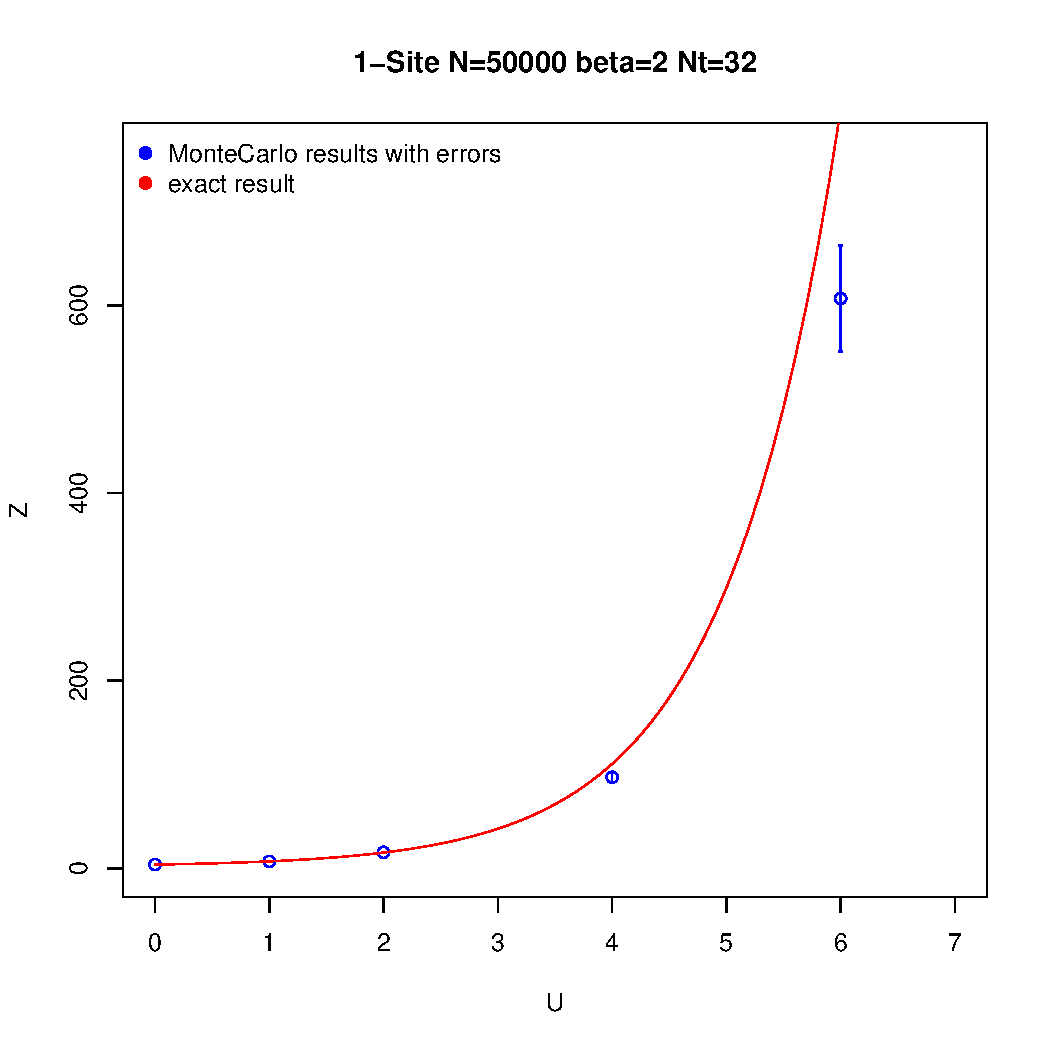
\includegraphics[width=0.5\linewidth]{figs/plot_Z1U}
	\caption[Scaling of Z with U]{This plot shows the scaling of $Z$ with $U$, while $\beta=2$, $N=50000$ and $N_t=32$}
	\label{fig:plotz1u}
\end{figure}

\begin{figure}[H]
	\centering
	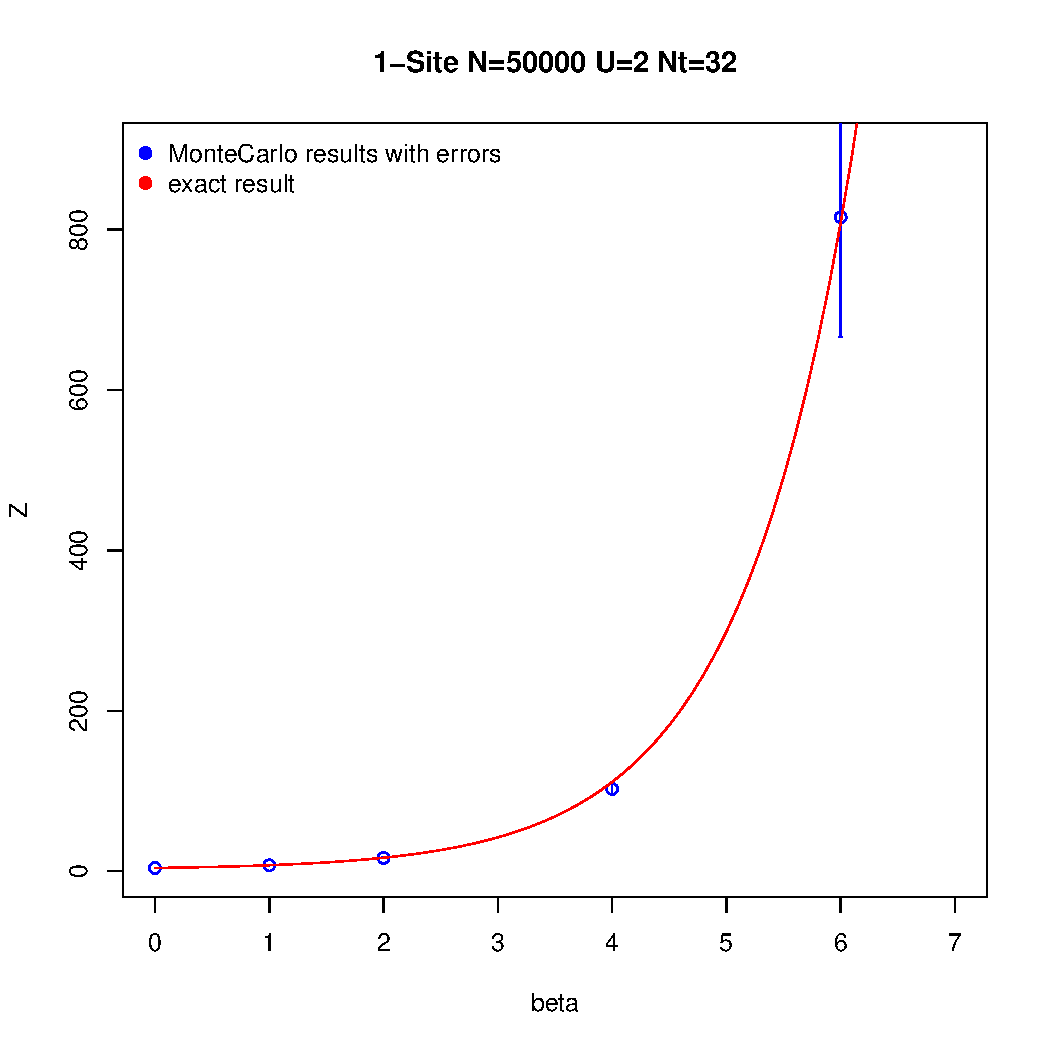
\includegraphics[width=0.5\linewidth]{figs/plot_Z1b}
	\caption[Scaling of Z with beta]{This plot shows the scaling of $Z$ with $\beta$, while $U=2$, $N=50000$ and $N_t=32$}
	\label{fig:plotz1b}
\end{figure}
The reason why they behave the same here is that, also in the algorithm (for the one site-model) $U$ and $\beta$ only appear together as $\tilde{U}=U\beta/N_t$. For more lattice sites $\beta$ will additionally be included in $\tilde{t}$.
Furthermore we see a decrease in accuracy for higher parameters, that can be compensated by increasing $N_t$, which reduces $\tilde{U}$. We assume that the greater variance of $\phi$, that comes with a greater $\tilde{U}$, reduces the precision as it broadens the possible $\phi$.
You can think about this physically as less change is happening between two measurements if you look more often or reduce the interaction.
\subsubsection{Correlator}
The correlator is defined from $0$ to $\beta$ as we have proposed continuous time it should obviously be periodic, with period $\beta$.
Figure 
\begin{figure}[H]
	\centering
	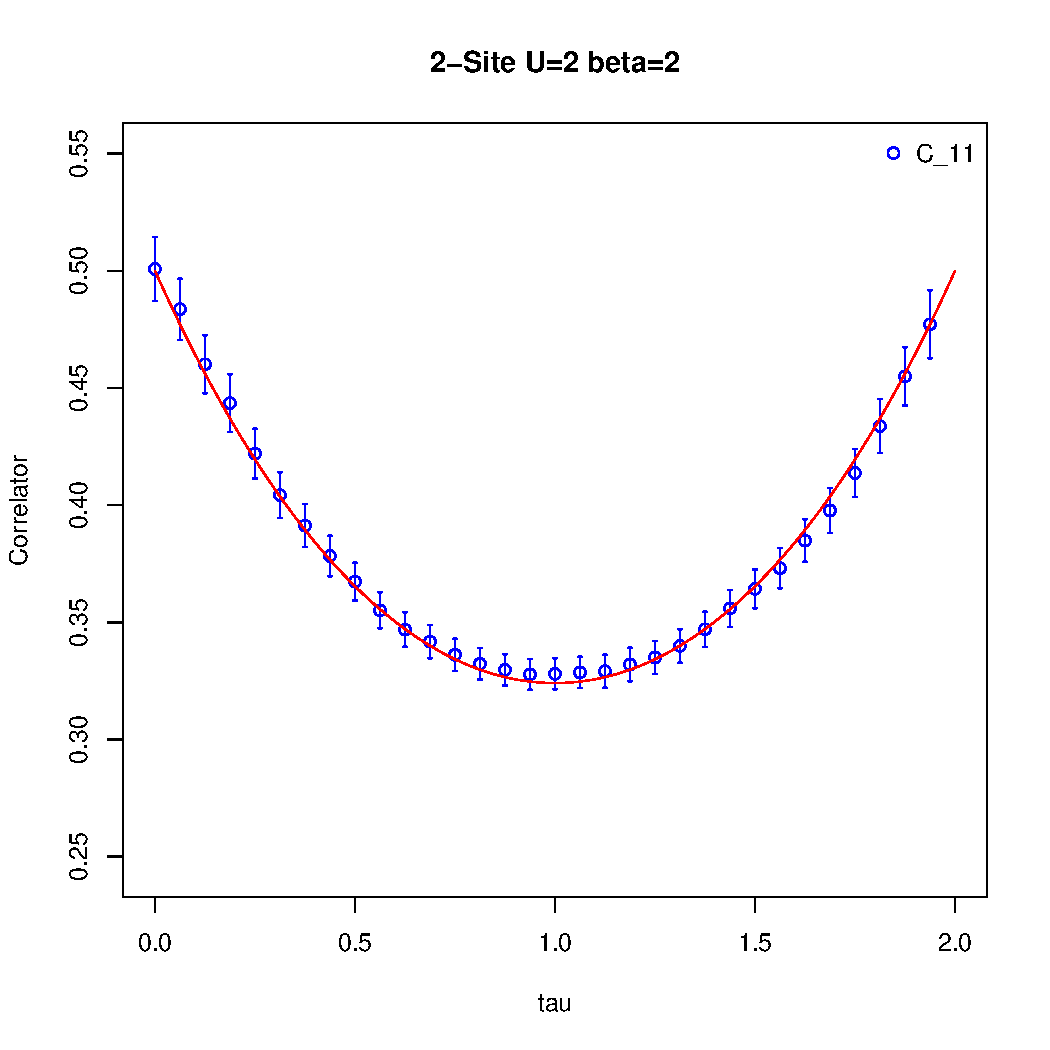
\includegraphics[width=0.5\linewidth]{figs/plot_C1t}
	\caption[Correlator 1 site]{This plot shows the correlator for the 1 site lattice, in comparison to its exact value. We used $N_t=32$ and $N=50000$}
	\label{fig:plotc1t}
\end{figure}
The calculated propagator fits very well to the exact value. Here the number of time slices was important too, but calculating the inverse of the fermion matrix slows down the calculation even more compared to the partition function and the scaling of the calculation time with $N_t$ gets even worse.
\subsection{Multiple lattice sites}
For multiple lattice sites the fermion matrix includes hopping terms